\section{Problem Statement}%
\label{sec:problem_statement}

\subsection{Toroidal Grid}%
\label{sub:toroidal_grid}

As stated on the AZsPCs website,\cite{zimmermann} the initial toroidal grid $O$ is defined as an $N\times N$ grid of unique tokens which ``wrap around'' (addressed in \ref{ssub:distance_metric}). For the sake of simplicity (and for reasons explained in \ref{ssub:distance_metric}), a token is of the form $\bm{IJ}$, where $\bm{I}$ and $\bm{J}$ are alphabetic representations of the indices of the rows and columns respectively, of a token, \emph{within $O$},\footnote{This is important because after rearranging the tokens, the identity of the token depends on its position within $O$, and not the rearranged position} eg.~$AC$ corresponds to the token in row 1, column 3 of $O$, $DF$ corresponds to the row 4, column 6 of $O$, etc. $O$ for $N=4$, is shown in \autoref{fig:toroidExample}. Tokens outside of the square grid represent tokens which ``wrap around'' the edges, resembling a toroidal surface as shown in \autoref{fig:wiki_toroid}.
\begin{figure}[htpb]
    \begin{subfigure}[t]{0.5\textwidth}
    \begin{center}
        \raisebox{0.4cm}{
        \includegraphics[width=0.7\textwidth]{images/Simple_Torus.pdf}}
    \caption{A Simple Toroid by Yassine Mrabet\cite{wiki_toroid}}
    \label{fig:wiki_toroid}
    \end{center}
    \end{subfigure}
    ~
    \begin{subfigure}[t]{0.5\textwidth}
    \begin{center}
    \toroidWarp{4}
    \caption{A $4\times 4$ \emph{intial} toroidal grid}%
    \label{fig:toroidExample}
    \end{center}
    \end{subfigure}
    \caption{Representations of a toroidal grid}
\end{figure}


\subsection{Evaluation Function}%
\label{sub:evaluation_function}

The goal of the challenge (and hence this essay) is to rearrange the tokens within $O$ to form a new grid $X$ that minimizes a loss function computed with the following procedure:
\begin{enumerate}
    \item For each unique pair of tokens\footnote{Comparisons between a token and itself do not affect the loss, since the distance between them is $0$, therefore, their inclusion or exclusion does not affect the computation} (eg. $[AA,BA]$ is equivalent to $[BA,AA]$, so $[BA,AA]$ is excluded), calculate the squared distance between them in the new grid,
    \item Multiply each of these by the squared distance between the pair of tokens within the original grid,
    \item Sum of all of these products
    \item Subtract a lower-bound corresponding to the value of $N$\footnote{Omitted here for brevity. Can be found at \cite{zimmermann}}
\end{enumerate}

\subsubsection{Distance Metric}%
\label{ssub:distance_metric}
To evaluate the loss function, a distance metric between two tokens must be established, which in turn necessitates defining the position of a token within a coordinate system.

\emph{The coordinate of a token is defined as the indices of the token within $X$.}

Note that within $O$, the coordinates, indices, and token representations are all equal.

 Let two two-dimensional coordinates $s_1=(x_1,y_1)$ and $s_2=(x_2,y_2)$, then the Euclidean distance $d_{euclid}$ is defined as
\begin{equation}
    \label{eq:euclid}
    d_{euclid}(s_1,s_2)=\sqrt{(x_2-x_1)^2+(y_2-y_1)^2}=\sqrt{(\Delta_{euclid} x)^2+(\Delta_{euclid} y)^2}.
\end{equation}

On a toroidal surface however, $\Delta x$ and $\Delta y$ can each have 2 possible values. A one-dimensional toroidal surface of length $N$ is illustrated in \autoref{fig:2distanceexample}. The corresponding possible values for $\Delta x$ are as follows:
\begin{align*}
    %\label{eq:naiveToroidDistance}
    \Delta_1(x)&=x_2-x_1 \\
    \Delta_2(x)&=(x_1-0)+(N-x_2)=x_1+N-x_2
\end{align*}

\begin{figure}[tpb]
    \centering
    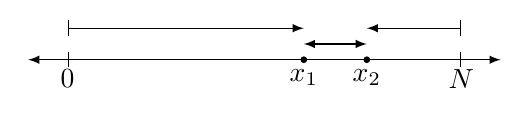
\begin{tikzpicture}
        \draw[latex-latex] (-3,0) -- (3,0);
        \draw[|-|] (-2.5,0) node[below] {$0$} -- (2.5,0) node[below] {$N$};
        %\draw[|-|] (-2.5,-0.5) -- node[below] {$N$} (2.5,-0.5);
        \filldraw (0.5,0) circle (1pt) node[below] {$x_1$};
        \filldraw (1.3,0) circle (1pt) node[below] {$x_2$};
        \draw[latex-latex] (0.5,0.2) -- (1.3,0.2);
        \draw[latex-|] (1.3,0.4) -- (2.5,0.4);
        \draw[|-latex] (-2.5,0.4) -- (0.5,0.4);
    \end{tikzpicture}
    \caption{A one-dimensional diagram of toroidal distance, with the two arrows representing two possible distances}%
    \label{fig:2distanceexample}
\end{figure}

To obtain a general equation which is applicable for $x_1>x_2$:
\begin{align*}
    \Delta_1(x)&=\lvert x_2-x_1 \rvert \\
    \Delta_2(x)&=\min{(x_1,x_2)}+N-\max{(x_1,x_2)}
    %\label{eq:absoluteToroidDistance}
\end{align*}
where $\lvert a\rvert$ is the absolute value of $a$, $\min{(a,b)}$ and $\max{(a,b)}$ are defined as the minimum and maximum between the values of $a$ and $b$ respectively, that is:
\begin{align*}
        \min{(a,b)}=
        \begin{cases}
            a&\text{if $a\leq b$}\\
            b&\text{if $a>b$}\\
        \end{cases}\qquad
        \max{(a,b)}=
        \begin{cases}
            a&\text{if $a\geq b$}\\
            b&\text{if $a<b$}\\
        \end{cases}
    %\label{eq:}
\end{align*}
$\min$ and $\max$ are used to determine the  ``left-most'' and the ``right-most'' coordinates.

One-dimensional toroidal distance is then defined as
\begin{align*}
    \Delta x=\min{(\Delta_1(x),\Delta_2(x))}.
\end{align*}

In two dimensions, the toroidal distance and squared toroidal distance are
\begin{align*}
    d(s_1,s_2)&=\sqrt{(\Delta x)^2+(\Delta y)^2} \\
    d^2(s_1,s_2)&=(\Delta x)^2+(\Delta y)^2
\end{align*}
From now on, \emph{distance} refers to $d^2$.

\subsubsection{Token Comparisons}%
\label{ssub:token_comparisons}
\begin{figure}[htpb]
    \centering
    \begin{subfigure}[t]{0.5\textwidth}
    \begin{center}
    \nestedToroid{2}
    \end{center}
    \caption{4-dimensional comparison with elements in the form $C(X)_{i,j,k,l}$}
    \label{fig:4dcomparison}
    \end{subfigure}%
    ~
    \begin{subfigure}[t]{0.5\textwidth}
    \begin{center}
    \twodcomparison{2}
    \end{center}
    \caption{2-dimensional comparison with elements in the form $C(X)_{m,n}$}
    \label{fig:2dcomparison}
    \end{subfigure}

    \caption{Tensors $C(X)$ representing comparison grids of an $N=2$ toroidal grid, where every element represents the distance between $X_{ij}$ and $X_{kl}$. Shaded cells denote unique comparisons.}%
    \label{fig:comparisonGrids}
\end{figure}

There are multiple ways of representing distances between all possible pairs of tokens, one of which is a 4-dimensional matrix (tensor) where every token within $X$ (first 2 dimensions), is compared to every token (next 2 dimensions). An example of the structure of the comparison for an $N=2$ grid is shown in \autoref{fig:4dcomparison}. The white boxes denote duplicate comparisons (eg. $
\begin{smallmatrix}
    BA\\ AA
\end{smallmatrix}
$ is identical to
$
\begin{smallmatrix}
    AA\\ BA
\end{smallmatrix}
$).

The dimensionality of the grid can be reduced\footnote{ie. to reduce the number of $\Sigma$s in \ref{ssub:loss_function_as_matrix_multiplications}} of the tensor can be reduced into a matrix: from $N\times N\times N\times N$ grid to $N^2\times N^2$, elements within the 4-dimensional tensor are of form $C(X)_{i,j,k,l}$, the 2-dimensional elements of the form $C(X)_{m,n}$. To do this conversion,
\begin{align*}
    m=(i-1)\times N+j &\implies m\div N=i-1 \text{ remainder } j\\
    n=(k-1)\times N+l &\implies n\div N=j-1 \text{ remainder } l
\end{align*}
$-1$ is to account for one-based indexing.

Both $C(X)_{i,j,k,l}$ and $C(X)_{m,n}$ represent the distance between tokens $\bm{IJ}$ and $\bm{KL}$ within $X$. The two-dimensional representation of \autoref{fig:4dcomparison} is shown in \autoref{fig:2dcomparison}.

From now on, let $C(X)$ refer to the two dimensional distance matrix.

\subsubsection{Loss Function in Matrix Form}%
\label{ssub:loss_function_as_matrix_multiplications}
Therefore the loss function for toroidal grid $X$ is equal to
\begin{align*}
    L(X)=\frac{1}{2}\sum_m^{N^2}\sum_n^{N^2}C(X)_{m,n}C(O)_{m,n}-c
\end{align*}
$c$ is the aforementioned lower-bound constant. Note that the diagonals of $C(O)$ and $C(X)$ are 0-valued, because they measure the distance between a token against itself. Therefore, to take into account only the unique distance measurements (ie. shaded cells) the factor of $\frac{1}{2}$ is added.
